\documentclass{scrreprt}

\usepackage{aligned-overset}
\usepackage{amsmath}
\usepackage{amsthm}
\usepackage{amssymb}
\usepackage{bm}
\usepackage[shortlabels]{enumitem}
\usepackage{hyperref}
\usepackage[utf8]{inputenc}
\usepackage{multicol}
\usepackage{mathtools}
\usepackage{pdflscape}
\usepackage{physics}
\usepackage{polynom}
\usepackage{tabularx}
\usepackage[table]{xcolor}
\usepackage{titling}
\usepackage{fancyhdr}
\usepackage{xfrac}
\usepackage{pgfplots}

\pgfplotsset{compat = newest}
\usetikzlibrary{arrows, arrows.meta}
\usetikzlibrary{calc}

\author{Karsten Lehmann \\ 4935758}
\date{WiSe 2024/25}
\title{Nachbereitungsaufgaben 11\\INF-B-110, Diskrete Strukturen}

\setlength{\headheight}{26pt}
\pagestyle{fancy}
\fancyhf{}
\lhead{\thetitle}
\rhead{\theauthor}
\lfoot{\thedate}
\rfoot{Seite \thepage}

\newcommand{\ggT}[0]{\text{ggT}}
\DeclarePairedDelimiter{\floor}{\lfloor}{\rfloor}

\begin{document}
\paragraph{N11}
\begin{enumerate}[(a)]
\item Zeichnen Sie jeweils ein Diagramm des Kantengraphen des $K_4$ und des Sterns
  \[
    S_5 = \qty(
      \qty\big{1, 2, 3, 4, 5},
      \qty{
        \qty\big{1, 5},
        \qty\big{2, 5},
        \qty\big{3, 5},
        \qty\big{4, 5}
      }
    )
  \]
  Bestimmen Sie für beide Kantengraphen das maximale $k \in \mathbb{N}$, so dass
  der Kantengraph $k$-fach zusammenhängend ist.

  \subparagraph{Lsg.} Die beiden Graphen sind

  \begin{minipage}{.45\textwidth}
    \begin{tikzpicture}
      \node[circle, draw, inner sep=0pt, minimum size=1mm,label=above left:{1}] (1) at (0,0) {};
      \node[circle, draw, inner sep=0pt, minimum size=1mm,label=above right:{2}] (2) at (2,0) {};
      \node[circle, draw, inner sep=0pt, minimum size=1mm,label=below right:{3}] (3) at (2,-2) {};
      \node[circle, draw, inner sep=0pt, minimum size=1mm,label=below left:{4}] (4) at (0,-2) {};

      \draw (3) -- (1) -- (2) -- (3) -- (4) -- (1);
      \draw (2) -- (4);

      \node at (0, -3) {$K_4$};
    \end{tikzpicture}
  \end{minipage}
  \begin{minipage}{.45\textwidth}
    \begin{tikzpicture}
      \node[circle, draw, inner sep=0pt, minimum size=1mm,label=above:{1}] (1) at (0,1) {};
      \node[circle, draw, inner sep=0pt, minimum size=1mm,label=right:{2}] (2) at (1,0) {};
      \node[circle, draw, inner sep=0pt, minimum size=1mm,label=below:{3}] (3) at (0,-1) {};
      \node[circle, draw, inner sep=0pt, minimum size=1mm,label=left:{4}] (4) at (-1,0) {};
      \node[circle, draw, inner sep=0pt, minimum size=1mm,label=above right:{5}] (5) at (0,0) {};

      \draw (5) -- (1);
      \draw (5) -- (2);
      \draw (5) -- (3);
      \draw (5) -- (4);

      \node at (-1, -2) {$S_5$};
    \end{tikzpicture}
  \end{minipage}

  und ihre Kantengraphen

  \begin{minipage}{.66\textwidth}
    \begin{tikzpicture}
      \node[circle, draw, inner sep=0pt, minimum size=1mm,label=right:{$\qty\big{1, 2}$}] (12) at ($(3, {sqrt(3)})$) {};
      \node[circle, draw, inner sep=0pt, minimum size=1mm,label=below:{$\qty\big{1, 3}$}] (13) at (2,0) {};
      \node[circle, draw, inner sep=0pt, minimum size=1mm,label=below:{$\qty\big{1, 4}$}] (14) at (0,0) {};
      \node[circle, draw, inner sep=0pt, minimum size=1mm,label=above:{$\qty\big{2, 3}$}] (23) at ($(2, {2*sqrt(3)})$) {};
      \node[circle, draw, inner sep=0pt, minimum size=1mm,label=above:{$\qty\big{2, 4}$}] (24) at ($(0, {2*sqrt(3)})$) {};
      \node[circle, draw, inner sep=0pt, minimum size=1mm,label=left:{$\qty\big{3, 4}$}] (34) at ($(-1, {sqrt(3)})$) {};

      \draw (12) -- (23) -- (34) -- (14) -- (24);
      \draw (12) -- (24) -- (23) -- (13) -- (12) -- (14) -- (13) -- (34) -- (24);


      \node at (-2, -1) {$L\qty(K_4)$};
    \end{tikzpicture}
  \end{minipage}
  \begin{minipage}{.33\textwidth}
    \begin{tikzpicture}
      \node[circle, draw, inner sep=0pt, minimum size=1mm,label=above left:{$\qty\big{1, 5}$}] (1) at (0,0) {};
      \node[circle, draw, inner sep=0pt, minimum size=1mm,label=above right:{$\qty\big{2, 5}$}] (2) at (2,0) {};
      \node[circle, draw, inner sep=0pt, minimum size=1mm,label=below right:{$\qty\big{3, 5}$}] (3) at (2,-2) {};
      \node[circle, draw, inner sep=0pt, minimum size=1mm,label=below left:{$\qty\big{4, 5}$}] (4) at (0,-2) {};

      \draw (1) -- (2) -- (3);
      \draw (1) -- (3);
      \draw (2) -- (4);
      \draw (1) -- (4) -- (3);

      \node at (-1, -4) {$L\qty(S_5)$};
    \end{tikzpicture}
  \end{minipage}

  In den folgenden Diagrammen sind für $L\qty(K_4)$ jeweils 4 paarweise unabhängige
  Pfade vom Knoten $\qty\big{2, 4}$ zu den Knoten $\qty\big{2. 3}$,
  $\qty\big{1. 2}$ und $\qty\big{1. 3}$ farblich hervorgehoben.
  Paarweise unabhängige Pfade zu den Knoten $\qty\big{3. 4}$ und $\qty\big{1, 4}$
  folgen durch Spiegelung der gegebenen Pfade an einer Achse durch die Knoten
  $\qty\big{2. 4}$ und $\qty\big{1. 3}$.

  Da jeder Knoten genau vier Kanten hat, ist offensichtlich, dass jeweils kein
  weiterer paarweise unabhängiger Pfad existieren kann.

  \begin{minipage}{.33\textwidth}
    \begin{tikzpicture}[scale=0.5]
      \node[circle, draw, inner sep=0pt, minimum size=1mm,label=right:{$\qty\big{1, 2}$}] (12) at ($(3, {sqrt(3)})$) {};
      \node[circle, draw, inner sep=0pt, minimum size=1mm,label=below right:{$\qty\big{1, 3}$}] (13) at (2,0) {};
      \node[circle, draw, inner sep=0pt, minimum size=1mm,label=below left:{$\qty\big{1, 4}$}] (14) at (0,0) {};
      \node[circle, draw, inner sep=0pt, minimum size=1mm,label=above right:{$\qty\big{2, 3}$}] (23) at ($(2, {2*sqrt(3)})$) {};
      \node[circle, draw, inner sep=0pt, minimum size=1mm,label=above left:{$\qty\big{2, 4}$}] (24) at ($(0, {2*sqrt(3)})$) {};
      \node[circle, draw, inner sep=0pt, minimum size=1mm,label=left:{$\qty\big{3, 4}$}] (34) at ($(-1, {sqrt(3)})$) {};

      \draw[line width=.75mm, blue] (24) -- (23);
      \draw[line width=.75mm, green] (24) -- (12) -- (23);
      \draw[line width=.75mm, red] (24) -- (14) -- (13) -- (23);
      \draw[line width=.75mm, pink] (24) -- (34) -- (23);
      \draw (34) -- (14) -- (12) -- (13) -- (34);
    \end{tikzpicture}
  \end{minipage}
  \begin{minipage}{.33\textwidth}
    \begin{tikzpicture}[scale=0.5]
      \node[circle, draw, inner sep=0pt, minimum size=1mm,label=right:{$\qty\big{1, 2}$}] (12) at ($(3, {sqrt(3)})$) {};
      \node[circle, draw, inner sep=0pt, minimum size=1mm,label=below right:{$\qty\big{1, 3}$}] (13) at (2,0) {};
      \node[circle, draw, inner sep=0pt, minimum size=1mm,label=below left:{$\qty\big{1, 4}$}] (14) at (0,0) {};
      \node[circle, draw, inner sep=0pt, minimum size=1mm,label=above right:{$\qty\big{2, 3}$}] (23) at ($(2, {2*sqrt(3)})$) {};
      \node[circle, draw, inner sep=0pt, minimum size=1mm,label=above left:{$\qty\big{2, 4}$}] (24) at ($(0, {2*sqrt(3)})$) {};
      \node[circle, draw, inner sep=0pt, minimum size=1mm,label=left:{$\qty\big{3, 4}$}] (34) at ($(-1, {sqrt(3)})$) {};

      \draw[line width=.75mm, blue] (24) -- (12);
      \draw[line width=.75mm, green] (24) -- (23) -- (12);
      \draw[line width=.75mm, red] (24) -- (34) -- (13) -- (12);
      \draw[line width=.75mm, pink] (24) -- (14) -- (12);
      \draw (23) -- (34) -- (14) -- (13) -- (23);
    \end{tikzpicture}
  \end{minipage}
  \begin{minipage}{.33\textwidth}
    \begin{tikzpicture}[scale=0.5]
      \node[circle, draw, inner sep=0pt, minimum size=1mm,label=right:{$\qty\big{1, 2}$}] (12) at ($(3, {sqrt(3)})$) {};
      \node[circle, draw, inner sep=0pt, minimum size=1mm,label=below right:{$\qty\big{1, 3}$}] (13) at (2,0) {};
      \node[circle, draw, inner sep=0pt, minimum size=1mm,label=below left:{$\qty\big{1, 4}$}] (14) at (0,0) {};
      \node[circle, draw, inner sep=0pt, minimum size=1mm,label=above right:{$\qty\big{2, 3}$}] (23) at ($(2, {2*sqrt(3)})$) {};
      \node[circle, draw, inner sep=0pt, minimum size=1mm,label=above left:{$\qty\big{2, 4}$}] (24) at ($(0, {2*sqrt(3)})$) {};
      \node[circle, draw, inner sep=0pt, minimum size=1mm,label=left:{$\qty\big{3, 4}$}] (34) at ($(-1, {sqrt(3)})$) {};

      \draw[line width=.75mm, blue] (24) -- (34) -- (13);
      \draw[line width=.75mm, green] (24) -- (23) -- (13);
      \draw[line width=.75mm, red] (24) -- (12) -- (13);
      \draw[line width=.75mm, pink] (24) -- (14) -- (13);
      \draw (34) -- (14) -- (12) -- (23) -- (34);
    \end{tikzpicture}
  \end{minipage}

  Da der Graph rotationssymmetrisch ist, gilt dies analog für die anderen
  Knoten und somit ist er nach Satz 67 der Vorlesung 4-fach zusammenhängend.


  Analog sind in den folgenden Diagrammen für $L\qty(S_5)$ jeweils 3 paarweise
  unabhängige Pfade vom Knoten $\qty\big{1, 5}$ zu den anderen 3 Knoten farblich
  hervorgehoben.
  Dabei ist offensichtlich, dass jeweils kein weiterer paarweise unabhängiger Pfad
  existieren kann.

  \begin{minipage}{.33\textwidth}
    \begin{tikzpicture}[scale=0.75]
      \node[circle, draw, inner sep=0pt, minimum size=1mm,label=above left:{$\qty\big{1, 5}$}] (1) at (0,0) {};
      \node[circle, draw, inner sep=0pt, minimum size=1mm,label=above right:{$\qty\big{2, 5}$}] (2) at (2,0) {};
      \node[circle, draw, inner sep=0pt, minimum size=1mm,label=below right:{$\qty\big{3, 5}$}] (3) at (2,-2) {};
      \node[circle, draw, inner sep=0pt, minimum size=1mm,label=below left:{$\qty\big{4, 5}$}] (4) at (0,-2) {};

      \draw[line width=.75mm, blue] (1) -- (2);
      \draw[line width=.75mm, green] (1) -- (3) -- (2);
      \draw (3) -- (4);
      \draw[line width=.75mm, red] (1) -- (4) -- (2);
    \end{tikzpicture}
  \end{minipage}
  \begin{minipage}{.33\textwidth}
    \begin{tikzpicture}[scale=0.75]
      \node[circle, draw, inner sep=0pt, minimum size=1mm,label=above left:{$\qty\big{1, 5}$}] (1) at (0,0) {};
      \node[circle, draw, inner sep=0pt, minimum size=1mm,label=above right:{$\qty\big{2, 5}$}] (2) at (2,0) {};
      \node[circle, draw, inner sep=0pt, minimum size=1mm,label=below right:{$\qty\big{3, 5}$}] (3) at (2,-2) {};
      \node[circle, draw, inner sep=0pt, minimum size=1mm,label=below left:{$\qty\big{4, 5}$}] (4) at (0,-2) {};

      \draw[line width=.75mm, blue] (1) -- (2) -- (3);
      \draw[line width=.75mm, green] (1) -- (3);
      \draw (2) -- (4);
      \draw[line width=.75mm, red] (1) -- (4) -- (3);
    \end{tikzpicture}
  \end{minipage}
  \begin{minipage}{.33\textwidth}
    \begin{tikzpicture}[scale=0.75]
      \node[circle, draw, inner sep=0pt, minimum size=1mm,label=above left:{$\qty\big{1, 5}$}] (1) at (0,0) {};
      \node[circle, draw, inner sep=0pt, minimum size=1mm,label=above right:{$\qty\big{2, 5}$}] (2) at (2,0) {};
      \node[circle, draw, inner sep=0pt, minimum size=1mm,label=below right:{$\qty\big{3, 5}$}] (3) at (2,-2) {};
      \node[circle, draw, inner sep=0pt, minimum size=1mm,label=below left:{$\qty\big{4, 5}$}] (4) at (0,-2) {};

      \draw[line width=.75mm, blue] (1) -- (4);
      \draw[line width=.75mm, green] (1) -- (2) -- (4);
      \draw (2) -- (3);
      \draw[line width=.75mm, red] (1) -- (3) -- (4);
    \end{tikzpicture}
  \end{minipage}

  Da auch dieser Graph rotationssymmetrisch ist, gilt dies analog für die 3 anderen
  Knoten und somit ist er nach Satz 67 der Vorlesung 3-fach zusammenhängend.


\item Für $n \in \mathbb{N}, n > 0$, wird der Graph $G_n = \qty\big(V_n, E_n)$
  betrachtet mit $V_n \coloneqq \qty(
    \qty\big(x, y)
    \:\middle|\:
    x, y \in \qty\big{0, \ldots, n - 1}
  )$ und $\qty{\qty\big(x_1, y_1), \qty\big(x_2, y_2)} \in E_n$ genau dann, wenn
  eine der folgenden Bedingungen gilt:
  \[
    y_1 = y_2 \text{ und }
    \qty(x_1 - x_2 \equiv 1 \qty\big(\mod n) \text{ oder } x_1 - x_2 \equiv -1 \qty\big(\mod n))
  \]
  \[
    x_1 = x_2 \text{ und }
    \qty(y_1 - y_2 \equiv 1 \qty\big(\mod n) \text{ oder } y_1 - y_2 \equiv -1 \qty\big(\mod n))
  \]
  \begin{enumerate}[(1)]
  \item Zeichnen Sie ein Diagramm von $G_2$ und ein Diagramm von $G_3$.

    \subparagraph{Lsg}. Es ist
    \[
      V_2 = \qty{
        \qty\big(0, 0),
        \qty\big(0, 1),
        \qty\big(1, 0),
        \qty\big(1, 1)
      }
    \]
    und
    \[
      E_2 = \qty{
        \qty{\qty\big(0, 0), \qty\big(0, 1)},
        \qty{\qty\big(0, 0), \qty\big(1, 0)},
        \qty{\qty\big(0, 1), \qty\big(1, 1)},
        \qty{\qty\big(1, 0), \qty\big(1, 1)}
      }
    \]
    \begin{tikzpicture}
      \node[circle, draw, inner sep=0pt, minimum size=1mm,label=above left:{$\qty\big(0, 0)$}] (1) at (0,0) {};
      \node[circle, draw, inner sep=0pt, minimum size=1mm,label=above left:{$\qty\big(0, 1)$}] (2) at (-1,-1) {};
      \node[circle, draw, inner sep=0pt, minimum size=1mm,label=above right:{$\qty\big(1, 0)$}] (3) at (1,-1) {};
      \node[circle, draw, inner sep=0pt, minimum size=1mm,label=below right:{$\qty\big(1, 1)$}] (4) at (0,-2) {};

      \draw (1) -- (2) -- (4) -- (3) -- (1);

      \node at (-1, -2.5) {$G_2$};
    \end{tikzpicture}

    Weiter ist
    \[
      V_2 = \qty{
        \qty\big(0, 0),
        \qty\big(0, 1),
        \qty\big(0, 2),
        \qty\big(1, 0),
        \qty\big(1, 1),
        \qty\big(1, 2),
        \qty\big(2, 0),
        \qty\big(2, 1),
        \qty\big(2, 2)
      }
    \]
    \begin{tikzpicture}
      \node[circle, draw, inner sep=0pt, minimum size=1mm,label=above:{$\qty\big(0, 0)$}] (1) at (0,0) {};
      \node[circle, draw, inner sep=0pt, minimum size=1mm,label=above left:{$\qty\big(0, 1)$}] (2) at (-1,-1) {};
      \node[circle, draw, inner sep=0pt, minimum size=1mm,label=above right:{$\qty\big(1, 0)$}] (3) at (1,-1) {};
      \node[circle, draw, inner sep=0pt, minimum size=1mm,label=left:{$\qty\big(1, 1)$}] (4) at (0,-2) {};
      \node[circle, draw, inner sep=0pt, minimum size=1mm,label=left:{$\qty\big(0, 2)$}] (5) at (-2,-2) {};
      \node[circle, draw, inner sep=0pt, minimum size=1mm,label=right:{$\qty\big(2, 0)$}] (6) at (2,-2) {};
      \node[circle, draw, inner sep=0pt, minimum size=1mm,label=left:{$\qty\big(2, 1)$}] (7) at (-1,-3) {};
      \node[circle, draw, inner sep=0pt, minimum size=1mm,label=right:{$\qty\big(1, 2)$}] (8) at (1,-3) {};
      \node[circle, draw, inner sep=0pt, minimum size=1mm,label=left:{$\qty\big(2, 2)$}] (9) at (0,-4) {};

      \draw (1) -- (2) -- (4) -- (3) -- (1);
      \draw (2) -- (5) -- (7) -- (4) -- (8) -- (6) -- (3);
      \draw (7) -- (9) -- (8);

      \node at (-1, -5) {$G_3$};
    \end{tikzpicture}
  \item Besitzt $G_3$ einen geschlossenen Eulerzug?
    Geben Sie einen solchen an oder begründen Sie, dass es keinen gibt.

    \subparagraph{Lsg.} Der Graph $G_3$ hat die 4 Knoten $\qty\big(0, 1)$,
    $\qty\big(1, 0)$, $\qty\big(2, 1)$ und $\qty\big(1, 2)$ mit dem ungeraden
    Grad 3.
    Nach Satz 76 der Vorlesung kann er somit keinen offenen Eulerzug besitzen.
  \end{enumerate}

\end{enumerate}
\end{document}
